\chapter{HH4b: Event Selection}
\label{chap:five}

In this search, the $\PX \to \PH\PH$ decay of a very heavy new resonance X would result in two highly Lorentz-boosted Higgs bosons.  Due to its large Lorentz boost, at least one of the decay products of each $H \to b\bar b$ decay are collimated, and reconstructed within a single AK8 jet. 
These are reconstructed using jet substructure and jet flavour-tagging techniques ~\cite{Butterworth:2008iy,Cooper:2013kia,Gouzevitch:2013qca} and, once they pass this selection, referred to as $\PH$ jets.

The standard model background consists mostly of multijet events, and is estimated using several control regions defined in the phase space of the masses and flavour-tagging discriminators of the two $\PH$ jets, and the $\PH\PH$ dijet invariant mass, allowing the background to be predicted over the entire $\mx$ range. 
The final event selection also contains a smaller amount of $t\bar{t}$+jets, which is modeled by 2D templates from the simulation; these templates are allowed to morph within uncertainties, and this morphing is governed by a number of nuisance parameters.
The dijet $M_{jj}$ mass distribution of the two leading Higgs-tagged jets corresponds to the invariant mass of the resonance searched for. 

The effectiveness of constraining the mass of each Higgs candidate to a $M_H$ window ~\cite{CMS-PAS-B2G-16-026} has been studied extensively. This technique was validated in the resolved and boosted searches~\cite{CMS-PAS-B2G-16-026}. One needs a variable which `corrects' the dijet invariant mass by the amount by which the individual H-jet masses are above or below the mass of the Higgs boson.  This approach is similar to a mass constraint in a $\chi^2$ fit but it does not bias the H-jet mass distribution. Therefore, the variable:
\begin{equation}
M^{red}_{jj} = M_{jj} - (M^1_{jet} - M_H) - (M^2_{jet} - M_H) \label{eq:mred}
\end{equation} 
is used to provide the best resolution of $M_{jj}$. 

The signal would appear as a peak in the $M_{jj}$ spectrum on top of a smooth background distribution. With this in mind, our analysis strategy is as follows:
\begin{itemize}
\item The signal region has two H tagged jets
\item We will be using the reduced mass, defined in Equation \ref{eq:mred}:
\item The main backgrounds are (i) QCD and (ii) $t\bar{t}$.  Their ratio depends on the H-tagger used (double-b or Deep AK8).
\item $t\bar t$+jets  is obtained from template-morphed MC shapes ($t\bar{t}$the nuisances are constrained in the fit to data)
\item QCD is obtained from H mass sidebands, and a ratio of pass and fail events, which is a smooth analytical function of $m_H$ and $m_{reduced}$ ($R_{p/f}$) (w.r.t. H-tag). This is accomplished by assigning one AK8 jet to pass the H-tagging first, and be `preselection side', and the other one is used in the 2DAlphabet background estimate and is called `Alphabet side'. 
\item Then an Alphabet style procedure is run in order to estimate the background and provide the $R_{p/f}$. The passing distribution in the signal region is modeled inside Combine by multiplying the failing distribution in data by the $R_{p/f}$.
\end{itemize}
%\newpage

\section{Event Selection\label{sec:EvtSel}}
\subsection{Fully Merged Topology}
Events passing the baseline triggers are further required to pass selection criteria close to the signal selection in the actual analysis:
\begin{itemize}
\item Leading two AK8 jets in the event with $\pt > 300 GeV$ and $|\eta| < 2.4$;
\item $\Delta \eta_{jj} < 1.3$ for the leading two AK8 jets, where $\Delta \eta_{jj} = |\eta_{1stFatJet} - \eta_{2ndFatJet}|$.
\end{itemize}
The details of these variables and selections are later described in Sections ~\ref{ss:JetSel} and ~\ref{ss:EvtSelMass}. 

For the $\Delta \eta_{jj}$ cut, the rationale is to suppress QCD, since the production of a heavy $X \to HH$ will be mostly central (as the bulk of the energy of the incoming partons would be used to create X), and thus the X will usually have low boost along the z axis. In contrast, in QCD, the valence quarks that glance off of each other and each go at very high eta to produce very large dijet invariant mass events. So this cut is a natural way to suppress QCD for very high masses of X. Events are required to have at least two jets, of which the two leading jets each need to have $\pt > 300 GeV$ and pseudorapidity $|\eta| < 2.4$. These two jets also need to be relatively close, $\Delta \eta_{jj} < 1.3$ in order to reduce any contribution from multijet events. A detailed study of this is given in Appendix B of \cite{CMS-PAS-B2G-16-026}.

\subsection{Jet kinematics selection\label{ss:JetSel}}

Individual particles are reconstructed using a particle flow (PF) algorithm ~\cite{PFPAS2009,CMS-PAS-PFT-10-001}, that combines the information from all the CMS detector components. Each such particle is referred to as a PF candidate. The five classes of PF candidates are muons, electrons, photons, and charged and neutral hadrons. \\

The anti-$k_t$ algorithm \cite{antiKtAlgorithm}, implemented in FASTJET \cite{Cacciari:2011ma}, clusters PF candidates ~\cite{PFPAS2009,CMS-PAS-PFT-10-001} into jets using a distance parameter $R = 0.8$ (referred to as AK8 jets). In order to mitigate the the effect of pileup on the different jet observables, we take advantage of the available pileup per particle identification (PUPPI) \cite{puppi}. This method uses the local shape information, event pileup properties, and tracking information together in order to compute a weight describing how pileup-like a particle is. 

The jet 4-momenta are corrected to account for the difference between expected and measured momentum at the particle level, using a standard CMS correction procedure described in \cite{CMS-PAS-JME-10-003}. We use the Jet Energy Correction (JEC) and Jet Energy Resolution (JER) corrections as implemented by the NanoAODtools JetMetUncertainties module \footnote{See here \url{https://github.com/cms-nanoAOD/nanoAOD-tools/tree/master/python/postprocessing/modules/jme}}.  All jets are further required to pass tight jet identification requirements provided by JetMET POG \footnote{\url{https://twiki.cern.ch/twiki/bin/view/CMS/JetMET}}.

Additionally, all events are required to pass all of the recommended \footnote{https://twiki.cern.ch/twiki/bin/viewauth/CMS/MissingETOptionalFiltersRun2\#Analysis\_Recommendations\_for\_ana} filters which account for, among other things, missing energy (MET).

\subsection{\texorpdfstring{\PH}{H} mass selection\label{ss:EvtSelMass}}

The masses of the two leading jets can be used to suppress the multijet and $\ttbar$ backgrounds. The jet-grooming algorithm called Soft Drop (cite) is used to remove the contributions from the underlying event (UE) activity and pileup, as well as remove soft and wide-angle radiation.  The jet grooming leaves the hard prongs from a H$\to b\bar b$ unaffected, whereas it strips away most of the soft radiation from a QCD shower.  As a result, the masses of QCD jets are pushed lower, whereas the jet masses from true Higgs jets are largely unchanged. The invariant mass, $M_{jj}$, is calculated. 
%A dedicated jet energy calibration correction is applied to the softdrop mass (cite). The correction is derived in two steps. First, a weight to account for $\pt$ dependence at the generator level (``gen correction'') is computed. Second, an additional weight is calculated to account for any $\pt$ and $\eta$ dependence between the reconstructed and generated softdrop mass (``reco correction'') after the ``gen correction'' has been applied. This difference between reconstructed and generated softdrop mass is a $5-10\%$ effect \cite{CMS-PAS-B2G-16-026}.

\subsection{Deep AK8 Mass De-correlated H Tagger\label{ss:deepAK8}}
In order to identify the two jets most likely to contain two b quarks, we use the deep AK8 mass decorrelated Hbb tagger, labeled \texttt{deep\_TagMDHbbvsQCD} \cite{CMS:2019gpd} in nanoAOD version 5. This tagger uses customized machine learning methods and what is called the ``DeepAK8'' algorithm using particle level information and secondary vertex information. Each is split into a separate ``set'' and a 1D CNN is applied to each set. The output of that is fed into a fully connected network to perform the jet classification. A mass prediction network is added for the version we are using because it is not desirable to use the ``DeepAK8'' algorithm when the mass distribution is used to discriminate between signal and background, as is in this analysis. Further details can be found in \cite{CMS:2019gpd}. 

We have made a $S/\sqrt{B}$ study in order to optimize the working points for this tagger, were we measure the data-to-MC efficiency SF ourselves. It should be noted that, in the optimization, the change in the H-jet selection affects also the `preselection' H-jet." At each signal MC mass point, $S/\sqrt{B}$ is calculated and the working points are chosen as the average over all the signal MC mass points. \footnote{In the previous analysis \cite{CMS-PAS-B2G-16-026}, $\tau_N$ was used to quantify the degree to which jet constituents could be arranged into N subjets. The ratio $\tau_{21} = \tau_2 / \tau_1$ was calculated for both jets and contributed a systematic uncertainty of $5-15\%$ \cite{CMS-PAS-B2G-16-026}. This requirement has been dropped for this analysis. We are using more modern taggers, \texttt{deepAK8MD\_HbbvsQCD} \cite{CMS:2019gpd} for example, which have the substructure information already included. Since this selection criteria is now redundant, we drop it and gain by reducing our systematic uncertainty. This study is documented in Appendix C.} We are using 0.9 as the tight working point and 0.8 as the loose working point\footnote{See the Appendix for previous studies on the working point.}.
We also show cutflow diagrams to illustrate the working point efficiencies for these points chosen. 
\begin{figure}[!htb]
	\centering
	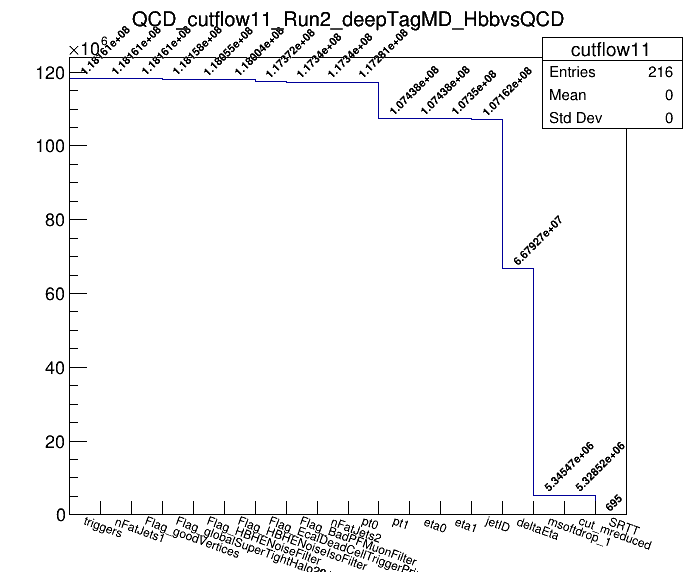
\includegraphics[width=0.8\textwidth]{Figures/QCD_cutflow11_Run2_deepTagMD_HbbvsQCD.png}
	\caption{Cutflow Diagram for Tight Tight QCD Selection}
	\label{fig:11CutflowqcdTT}
\end{figure}
\begin{figure}[!htb]
	\centering
	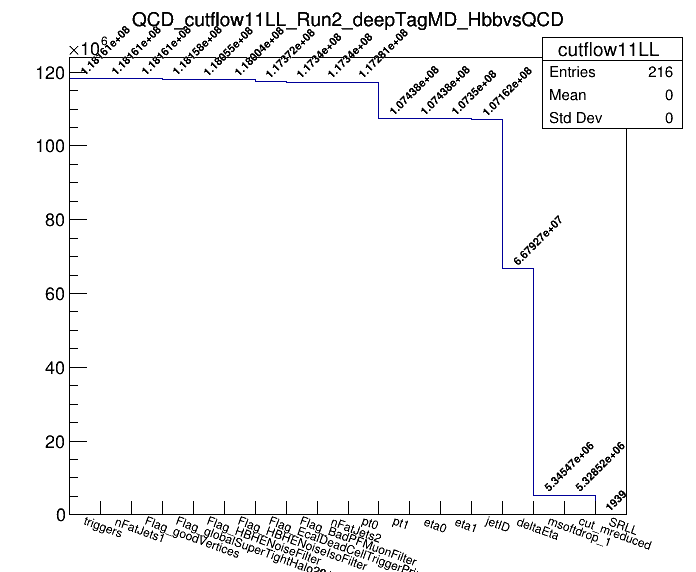
\includegraphics[width=0.8\textwidth]{Figures/QCD_cutflow11LL_Run2_deepTagMD_HbbvsQCD.png}
	\caption{Cutflow Diagram for Loose Loose QCD Selection}
	\label{fig:11CutflowqcdLL}
\end{figure}
\begin{figure}[!htb]
	\centering
    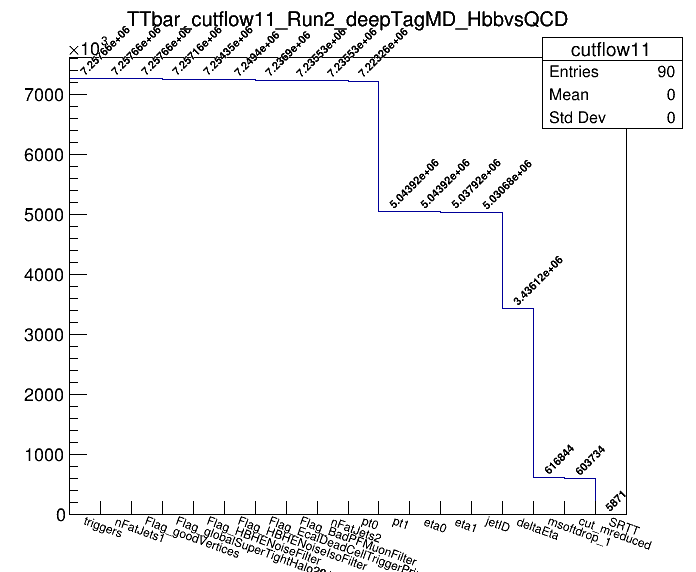
\includegraphics[width=0.8\textwidth]{Figures/ttbar_cutflow11_Run2_deepTagMD_HbbvsQCD.png}
	\caption{Cutflow Diagram for Tight Tight $\ttbar$ Selection}
	\label{fig:11CutflowttTT}
\end{figure}
\begin{figure}[!htb]
	\centering
    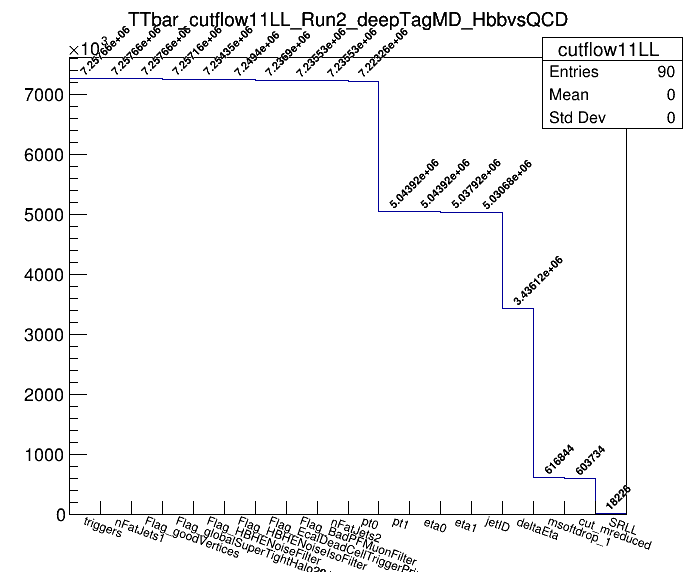
\includegraphics[width=0.8\textwidth]{Figures/ttbar_cutflow11LL_Run2_deepTagMD_HbbvsQCD.png}
	\caption{Cutflow Diagram for Loose Loose $\ttbar$ Selection}
	\label{fig:11CutflowttLL}
\end{figure}
\begin{figure}[!htb]
	\centering
    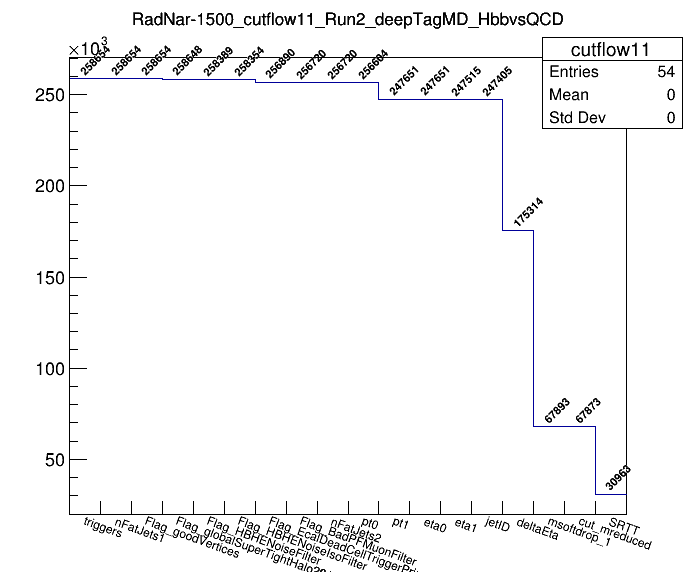
\includegraphics[width=0.8\textwidth]{Figures/radnar1500_cutflow11_Run2_deepTagMD_HbbvsQCD.png}
	\caption{Cutflow Diagram for Tight Tight Radion 1500 GeV Selection}
	\label{fig:11CutflowsigTT}
\end{figure}
\begin{figure}[!htb]
	\centering
    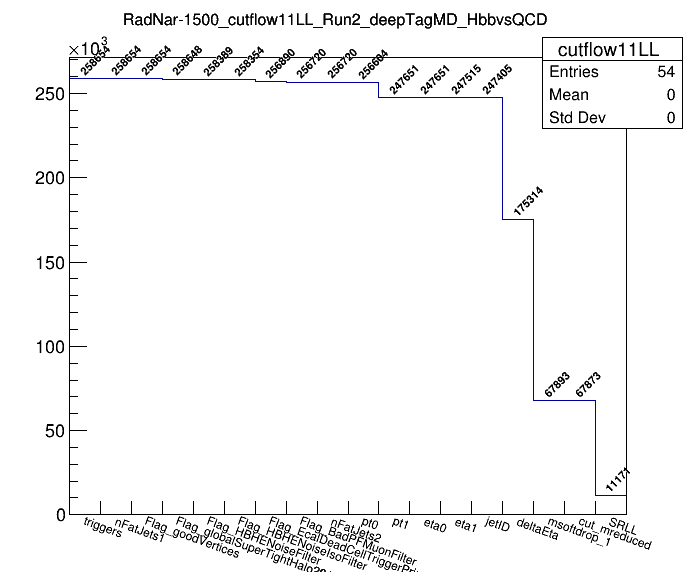
\includegraphics[width=0.8\textwidth]{Figures/radnar1500_cutflow11LL_Run2_deepTagMD_HbbvsQCD.png}
	\caption{Cutflow Diagram for Loose Loose Radion 1500 GeV Selection}
	\label{fig:11CutflowsigLL}
\end{figure}

% \begin{center}
% \begin{tabular}{ |c|c| } 
%  \hline
%  Background & Selection Efficiency \\ 
%  \hline
%  QCD & $> 99$\% \\ 
%  $\ttbar$ & $99.02$\% \\ 
%  RadNar-1500 & $54.38$\% \\   
%  \hline
% \end{tabular}
% \end{center}
\clearpage
\subsection{Boosted Event Selection\label{sec:EvtSel1p1}} 
The event selection follows the same as the trigger above but adding the following criteria:
\begin{itemize}
\item The soft drop mass of the two jets are $110 < M_{softdrop} < 140 GeV$, with all necessary jet mass corrections applied 
\item The dijet invariant mass, $M^{red}_{jj}$, $> 750$.
\end{itemize}
The soft drop mass window was optimized by making preliminary limits for three different windows. The results are shown in Figure \ref{fig:sdmasswindow} 
\begin{figure}[!htb]
	\centering
	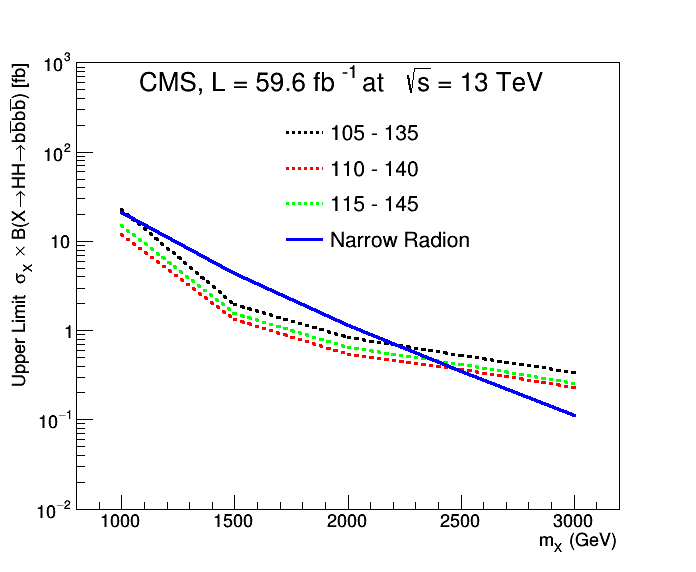
\includegraphics[width=0.8\textwidth]{Figures/limits_HH_combine_59.6fb_softdropwindow_limit_comparison_RadNar.png}
	\caption{Preliminary limits used to optimize the soft drop mass window.}
	\label{fig:sdmasswindow}
\end{figure}

\subsection{Identification of Higgs jets in boosted analysis\label{sec:EvtSelBoostedtagging}}
For the boosted analysis, events are required to pass the above selection criteria. The double b-tagger described in Section~\ref{ss:deepAK8} is used to identify the boosted Higgs jet in the boosted analysis. We then split the candidate events into tight-tight (TT) and loose-loose (LL) pass and fail regions. The algorithm to do this is as follows:
The 2D Alphabet method, with the signal region blinded, is then used to obtain the background estimate in the signal region. The possible combinations taken into account are:
\begin{itemize}
\item TT Pass: Both H-jets pass the tight operating point;
\item TT Fail: The leading H-jet fails the tight operating point and the subleading passes.
\item LL Pass: Both H-jets pass the loose working point but both fail the tight working point. This also means that if one jet passes the loose working point and the other passes the tight working point, the event will be classified as LL.
\item LL Fail: The leasing H-jet fails the loose operating point and the subleading passes the loose operating point. The subleading H-jet must also fail the tight working point.
\end{itemize}
\begin{figure}[!htb]
	\centering
	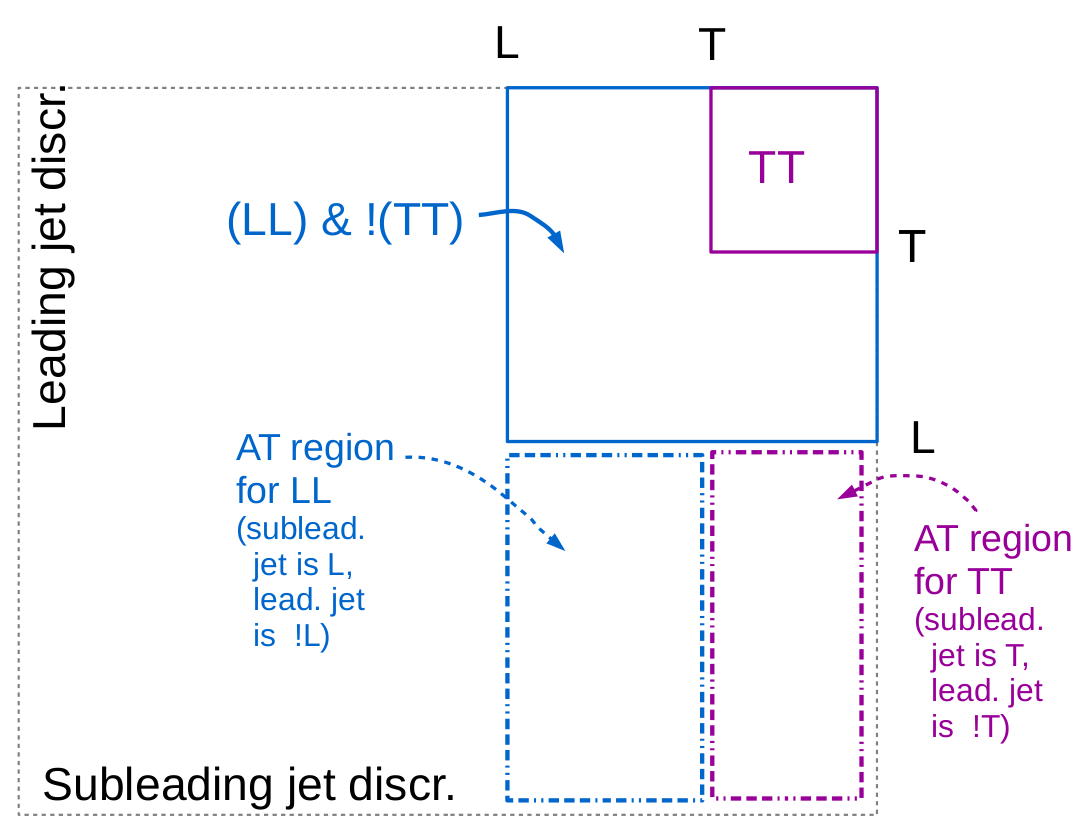
\includegraphics[width=0.6\textwidth]{Figures/splitting.png}
	\caption{A pictorial representation of the semaphoring of Loose Loose and Tight Tight events.}
	\label{fig:splitting}
\end{figure}
\clearpage

\subsection{MC distributions before applying Selections\label{ss:beforeDist}}
The kinematic variables before the application of $H \to bb$ tagger(s), are shown in Figs.\ref{fig:prePtlead} through \ref{fig:preMred}. Here, the $\ttbar$ distributions are normalized to luminosity where signal and qcd is normalized to $\ttbar$ for ease of viewing. Also, the difference between TT and LL distributions is in the weight used for each. Since the deepTagMD$\_$HbbvsQCD tagger has not been applied yet, we do not split the plots into Tight Tight and Loose Loose.

\begin{figure}[!htb]
	\centering
	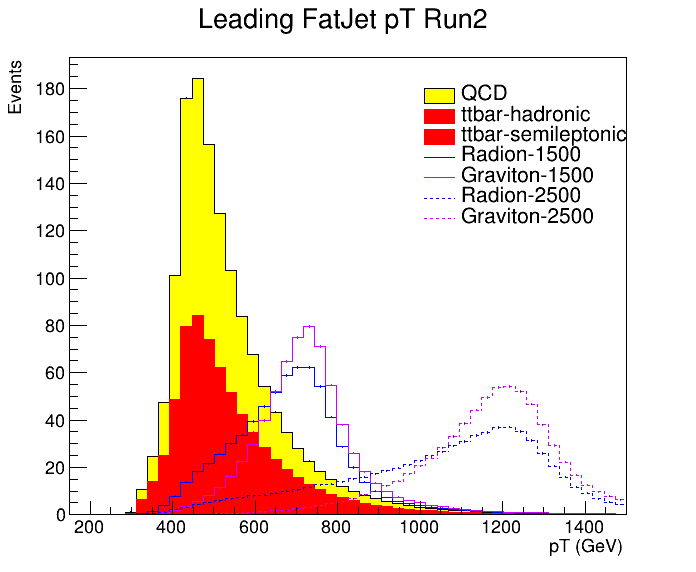
\includegraphics[width=0.4\textwidth]{Figures/pt0TT_Run2_deepTagMD_HbbvsQCD.png}
	% \includegraphics[width=0.4\textwidth]{Figures/pt021_Run2_deepTagMD_HbbvsQCD.png}
	\caption{Pre deepTagMD$\_$HbbvsQCD selection $p_T$ distribution of leading fat jet}
	\label{fig:prePtlead}
\end{figure}
\begin{figure}[!htb]
	\centering
	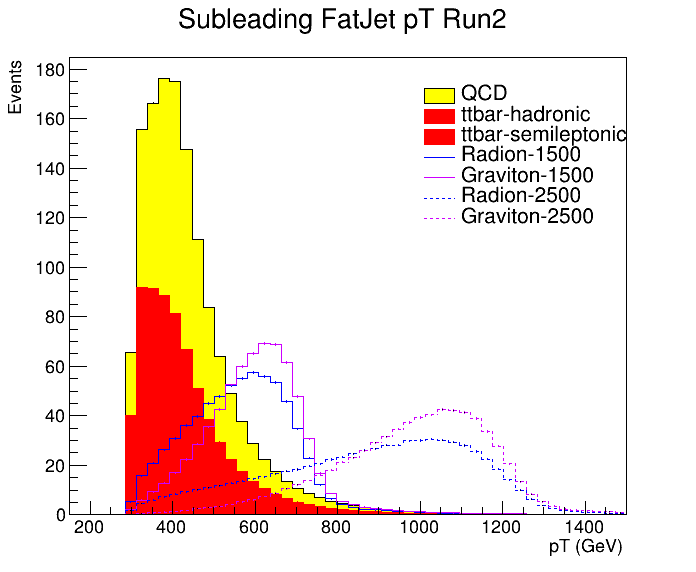
\includegraphics[width=0.4\textwidth]{Figures/pt1TT_Run2_deepTagMD_HbbvsQCD.png}
	\caption{Pre deepTagMD$\_$HbbvsQCD selection $p_T$ distribution of subleading fat jet}
	\label{fig:prePtsub}
\end{figure}
% \begin{figure}[!htb]
% 	\centering
% 	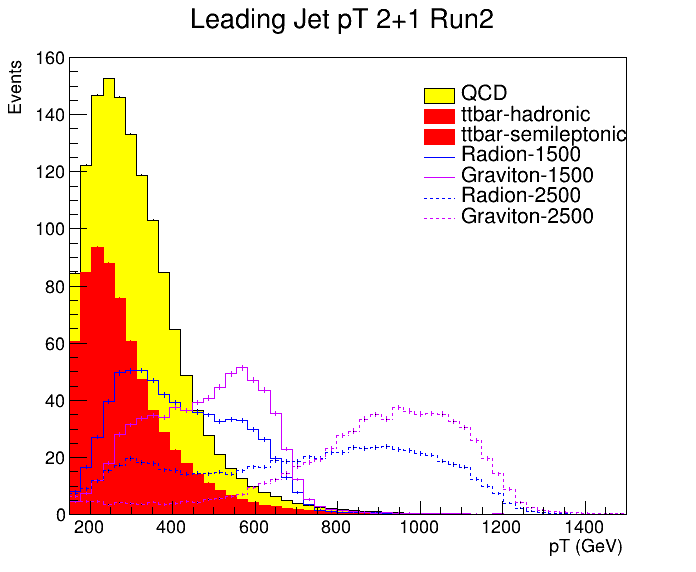
\includegraphics[width=0.4\textwidth]{Figures/bpt021_Run2_deepTagMD_HbbvsQCD.png}
% 	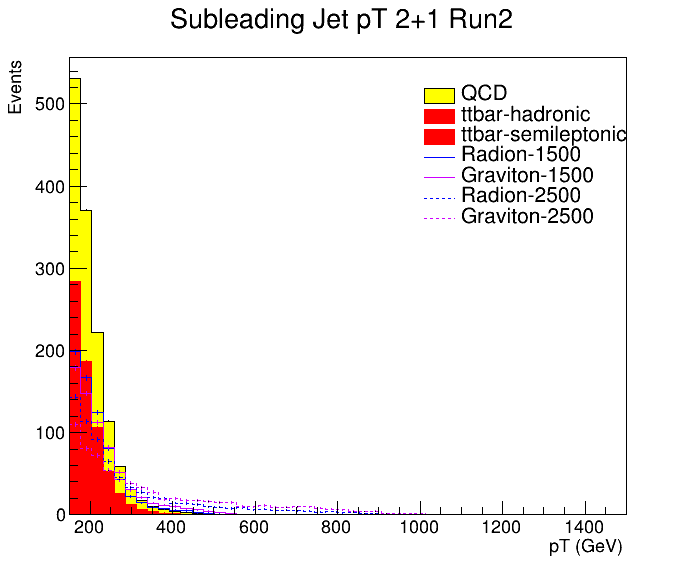
\includegraphics[width=0.4\textwidth]{Figures/bpt121_Run2_deepTagMD_HbbvsQCD.png}
% 	\caption{Pre deepTagMD$\_$HbbvsQCD selection $p_T$ distribution of leading and subleading jet for Semi-resolved.}
% 	\label{fig:prePtlead}
% \end{figure}
\begin{figure}[!htb]
	\centering
	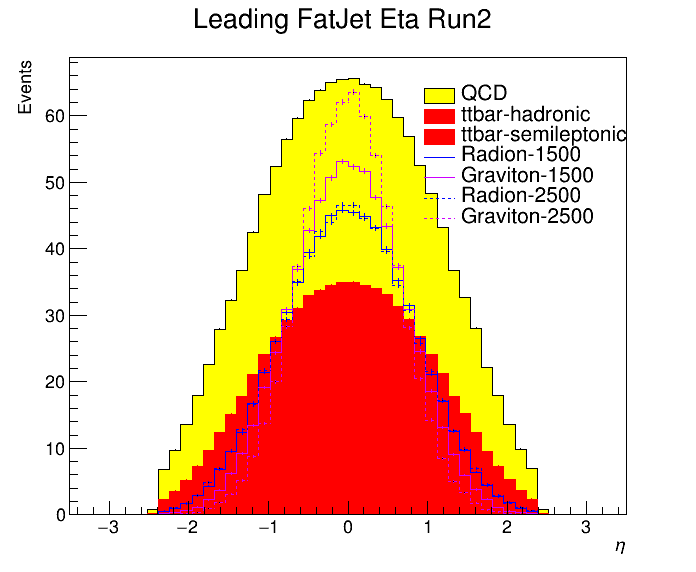
\includegraphics[width=0.4\textwidth]{Figures/eta0TT_Run2_deepTagMD_HbbvsQCD.png}
	% \includegraphics[width=0.4\textwidth]{Figures/eta021_Run2_deepTagMD_HbbvsQCD.png}
	\caption{Pre deepTagMD$\_$HbbvsQCD selection $\eta$ distribution of leading fat jet}
	\label{fig:preEtalead}
\end{figure}
\begin{figure}[!htb]
	\centering
	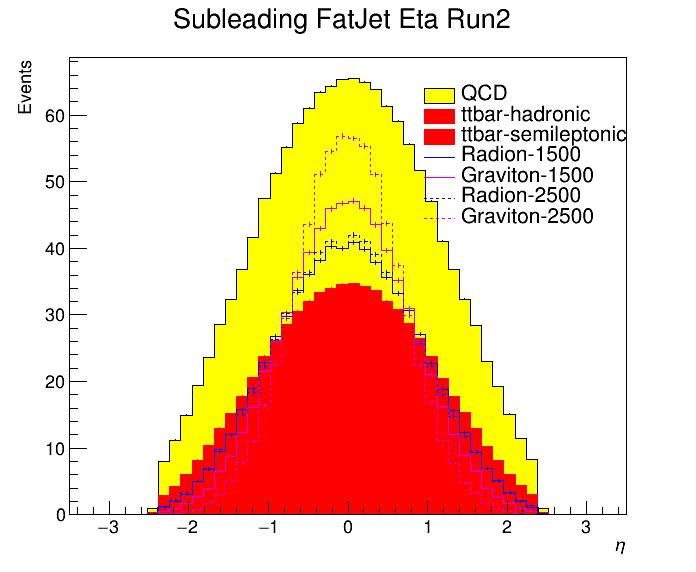
\includegraphics[width=0.4\textwidth]{Figures/eta1TT_Run2_deepTagMD_HbbvsQCD.png}
	\caption{Pre deepTagMD$\_$HbbvsQCD selection $\eta$ distribution of subleading fat jet}
	\label{fig:preEtasub}
\end{figure}
% \begin{figure}[!htb]
% 	\centering
% 	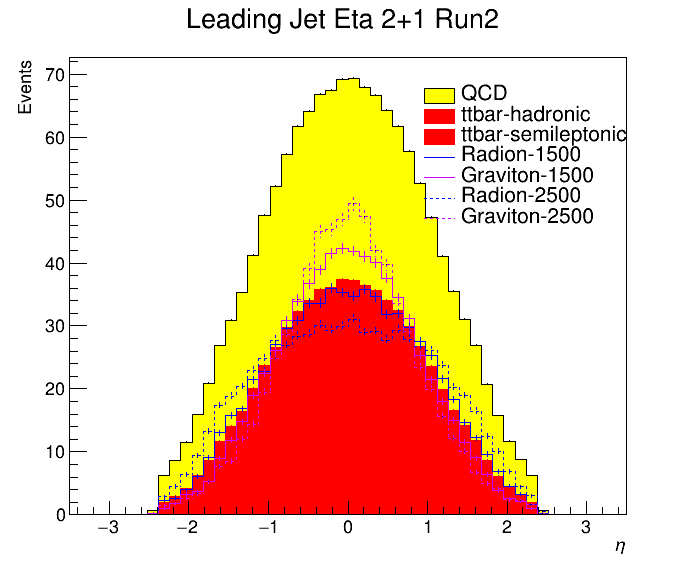
\includegraphics[width=0.4\textwidth]{Figures/beta021_Run2_deepTagMD_HbbvsQCD.png}
% 	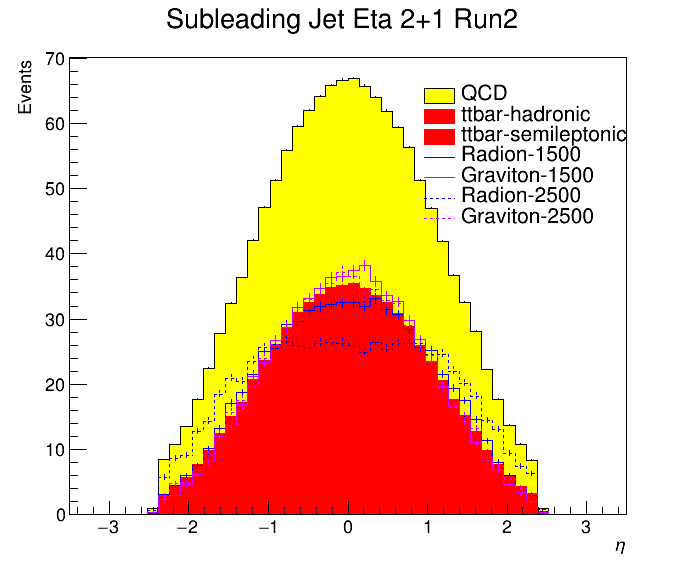
\includegraphics[width=0.4\textwidth]{Figures/beta121_Run2_deepTagMD_HbbvsQCD.png}
% 	\caption{Pre deepTagMD$\_$HbbvsQCD selection $\eta$ distribution of leading and subleading jet for Semi-resolved.}
% 	\label{fig:prePtlead}
% \end{figure}
\begin{figure}[!htb]
	\centering
	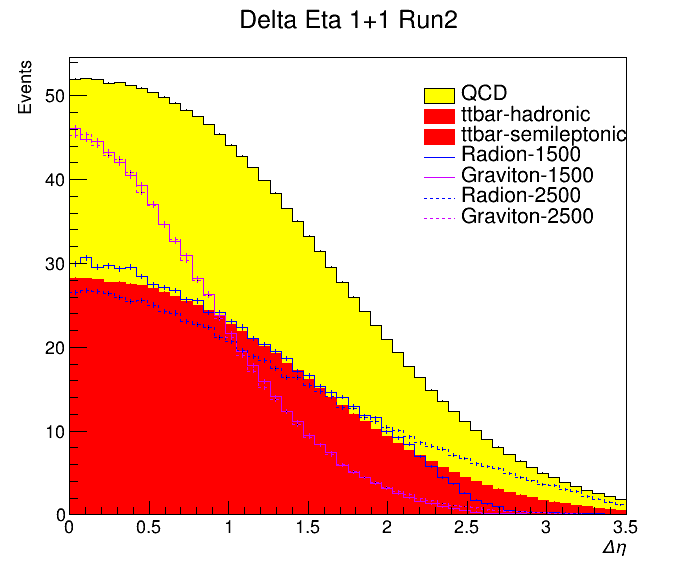
\includegraphics[width=0.4\textwidth]{Figures/deltaEtaTT_Run2_deepTagMD_HbbvsQCD.png}
	% 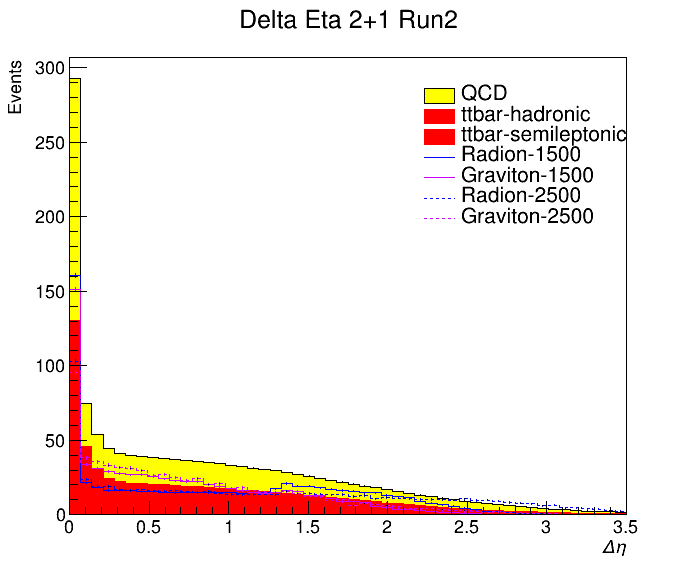
\includegraphics[width=0.4\textwidth]{Figures/deltaEta21_Run2_deepTagMD_HbbvsQCD.png}
	\caption{Pre deepTagMD$\_$HbbvsQCD selection $\Delta \eta$ distribution}
	\label{fig:predeltaEta}
\end{figure}
\begin{figure}[!htb]
	\centering
	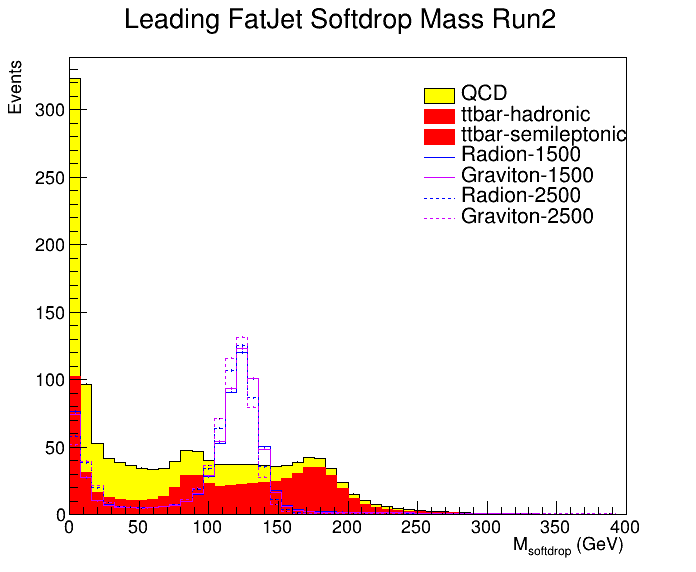
\includegraphics[width=0.4\textwidth]{Figures/msd0TT_Run2_deepTagMD_HbbvsQCD.png}
	% 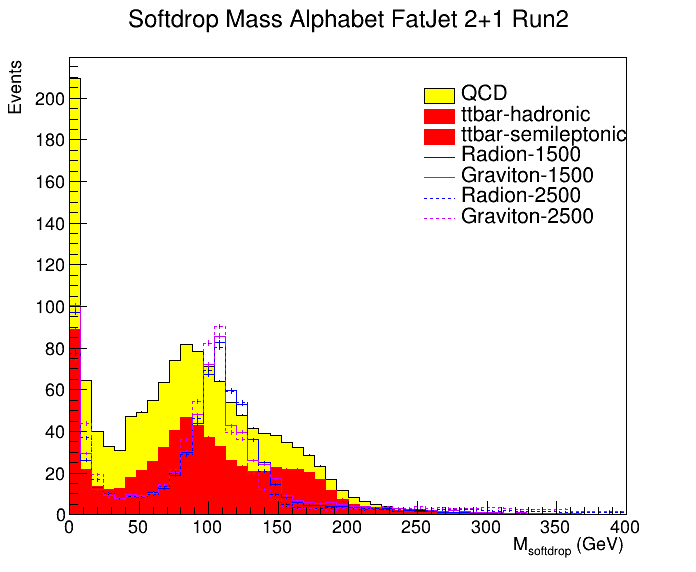
\includegraphics[width=0.4\textwidth]{Figures/msd021_Run2_deepTagMD_HbbvsQCD.png}
	\caption{Pre deepTagMD$\_$HbbvsQCD selection $m_{j}$ distribution}
	\label{fig:premsd0}
\end{figure}
\begin{figure}[!htb]
	\centering
	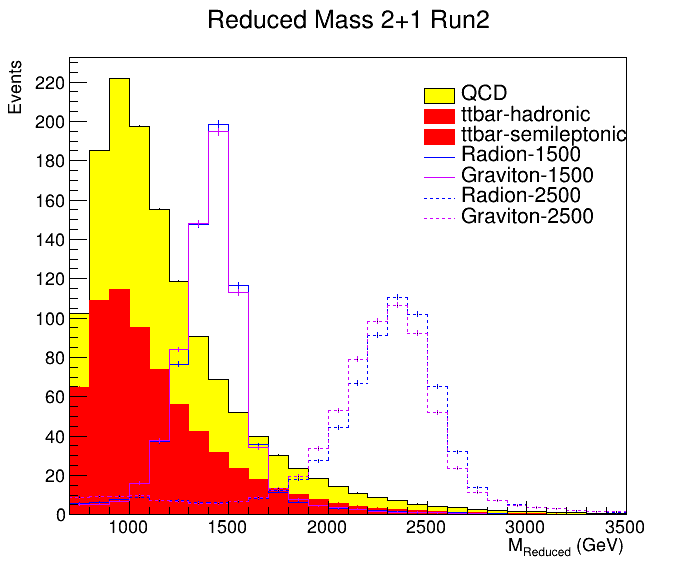
\includegraphics[width=0.4\textwidth]{Figures/mred21_Run2_deepTagMD_HbbvsQCD.png}
	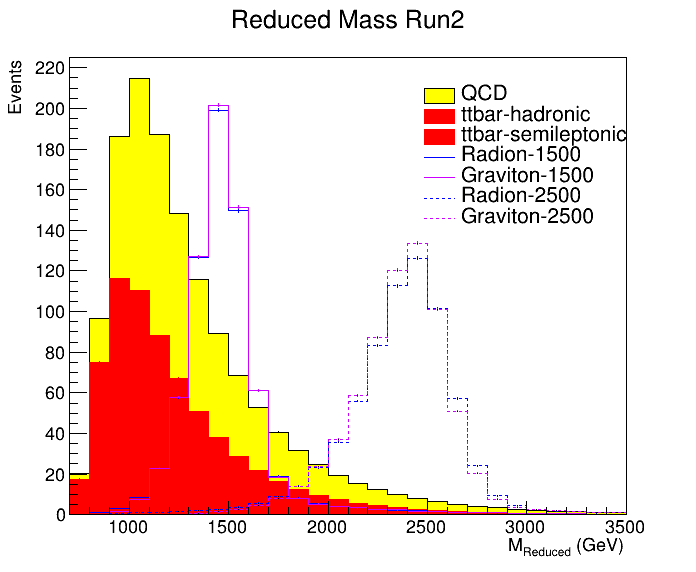
\includegraphics[width=0.4\textwidth]{Figures/mredTT_Run2_deepTagMD_HbbvsQCD.png}
	\caption{Pre deepTagMD$\_$HbbvsQCD selection $m_{jj}$ distribution}
	\label{fig:preMred}
\end{figure}

\section{Semi-Resolved Topology\label{app:2p1}}

The semi-resolved case bridges the gap between the fully resolved analysis for HH $\rightarrow$ 4b~\cite{CMS_AN_2015-108} and the boosted analysis, presented in Section \ref{sec:EvtSel}. It assumes one H is boosted enough to be contained within an AK8 jet with two subjets and the other H is not, resulting in two AK4 jets, one for each b quark. We use techniques similar to the boosted analysis to identify the boosted Higgs and use techniques similar to the resolved analysis to identify the two resolved b-jets. For this case, the mass range is sensitive as well.

\subsection{Event Selection\label{sec:EvtSel2p1}} 
The jet kinematics selection is the same as that of the boosted analysis for the AK8 jet. The AK4 jets also have a kinematic selection. Events are required to have:
\begin{itemize}
\item 2 AK4 jets, $p_{T}$ $>$ 30 GeV, $\etaj < 2.0$, deep Jet $>$ medium WP by year [2016:0.3093 ,2017:0.3033 ,2018:0.2770]
\item 1 AK8 jet, $p_{T}$ $>$ 300 GeV, $\etaj < 2.4$%, $\Delta$R (AK8 jet, AK4 jets) $>$ 1.5
% \item $\Delta \eta_{jjj} < 1.3$ for the leading AK8 jet and two AK4 jets, where $\Delta \eta_{jjj} = |\eta_{1stFatJet} -(\eta_{1stJet} + \eta_{2ndJet})|$.
\item Trijet mass, defined and studied in \cite{CMS-PAS-B2G-16-026}, $> 200.0$ GeV
%\item $\Delta$R of nearest unselected AK4 jet $> 1.0$ 
\end{itemize}
We choose the appropriate AK4 jets by requiring that the AK8 jet is at least $\Delta R > 0.8$ away from the candidate AK4 jets. We also require that the AK4 jets are $\Delta \phi > \frac{\pi}{2}$ away from the candidate AK8 jet in order to guarantee that the AK4 jets are in a different hemisphere than the AK8 jet. For each candidate AK4 jet pair, we require that the jets are within $\Delta R < 1.5$. After this, the dijet mass is required to be between 90 and 140 GeV, and the DeepAK8-discriminant is used to determine the control region (DeepAK8 discriminant $<$ 0.9, Tight WP) and signal region (DeepAK8 discriminant $>$ 0.9). 

\subsection{Identification of Higgs jets in semi-resolved analysis\label{sec:EvtSelBtagging}}
For the semi-resolved analysis, events are required to have at least one jet as described Section~\ref{sec:EvtSel}. The DeepAK8-tagger described in Section~\ref{sec:EvtSel} is used to identify the boosted Higgs jet in the semi-resolved analysis, requiring the fatjet pass the working point of DeepAK8 discriminant $>$ 0.9. 
We show the cutflow diagram here.
\begin{figure}[!htb]
	\centering
	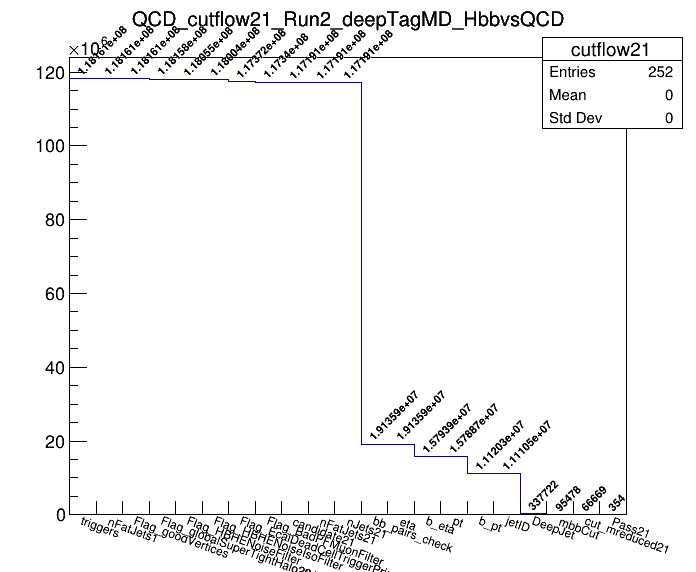
\includegraphics[width=0.8\textwidth]{Figures/QCD_cutflow21_Run2_deepTagMD_HbbvsQCD.png}
	\caption{Cutflow Diagram for Semi-resolved for QCD Selection}
	\label{fig:21Cutflowqcd}
\end{figure}
\begin{figure}[!htb]
	\centering
    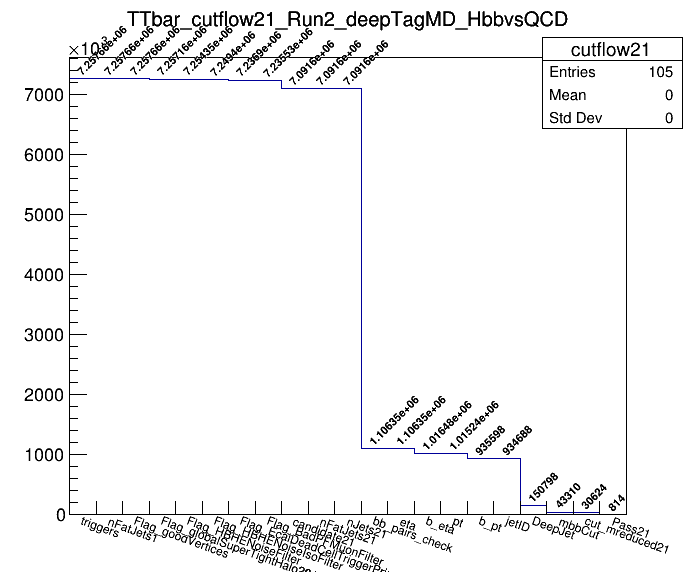
\includegraphics[width=0.8\textwidth]{Figures/ttbar_cutflow21_Run2_deepTagMD_HbbvsQCD.png}
	\caption{Cutflow Diagram for Semi-resolved for $\ttbar$ Selection}
	\label{fig:21Cutflowtt}
\end{figure}
\begin{figure}[!htb]
	\centering
    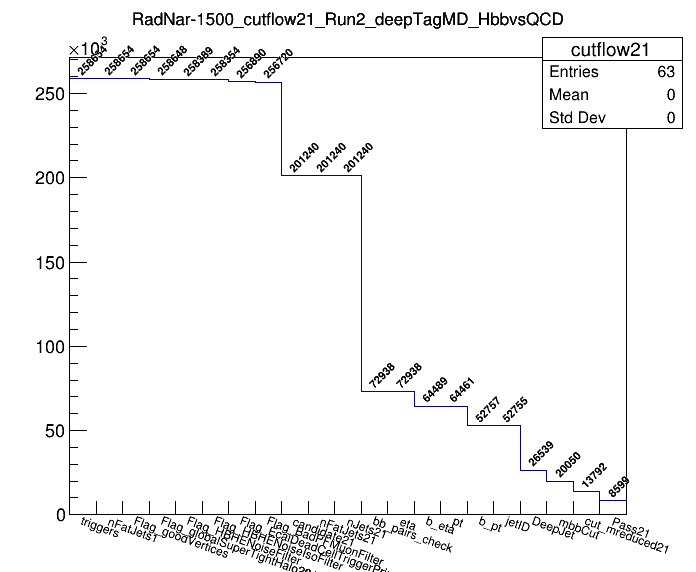
\includegraphics[width=0.8\textwidth]{Figures/radnar1500_cutflow21_Run2_deepTagMD_HbbvsQCD.png}
	\caption{Cutflow Diagram for Semi-resolved for Radion 1500 GeV Selection}
	\label{fig:21Cutflowsig}
\end{figure}

The invariant mass of all three jets is used in the same way as the reduced dijet mass is used for the boosted analysis and is given by:
\begin{equation}
M^{red}_{jjj} = M_{jjj} - (M_{Fatjet} - M_H) - (M_{jj(Ak4jets)} - M_H) \label{eq:mred2p1}
\end{equation} 